\section{Experiments}\label{sec:exps}
%%%%%%%%%%%%%%%%%%%%%%%%%%%%%%%%%%%%%
%
\subsection{Datasets}\label{sec:exps_datasets} 
%
We evaluate Okapi on three datasets taken from the WILDS 2.0 benchmark \citep{SagWeiLeeGaoetal22}. 
%
These span a variety of modalities and tasks, allowing us to showcase the generality of our
proposed method (Okapi): \textbf{iWildCam} (images, multiclass classification), \textbf{PovertyMap}
(multispectral images, regression), and \textbf{CivilComments} (text, binary classification). 
%
Details of each dataset can be found in Appendix~\ref{appx:datasets}.
%
\subsection{Image experiments}
%
\import{okapi}{tables/iw_pm_results.tex}
%
Results of our image-data experiments are summarised in Table~\ref{tab:iw_pm_results}. 
%
Due to spacial constraints, we defer the full set of results, including those for the `offline'
(\wrt{} the matching) version of Okapi to Appendix~\ref{appx:ext_results}. 
%
For both datasets in question, we use the same metrics as \citet{SagWeiLeeGaoetal22}: macro-F1 for
iWildCam and worst-group (with the group defined as urban (U) vs. rural (R)) Pearson correlation
for Poverty Map. 
%
For completeness, we include mean squared error (MSE) as a secondary metric for the latter dataset.
%
Following \citet{SagWeiLeeGaoetal22}, we compute the mean and standard deviation (shown in
parentheses) over multiple runs for both \ac{ID} and \ac{OOD} test sets, with these runs conducted
with 3 different random seeds and 5 pre-defined cross-validation folds for iWildCam and PovertyMap,
respectively.

We compare Okapi against two baselines, \ac{ERM} and FixMatch \citep{sohn2020fixmatch},
both according to our re-implementation and according to the original implementation given in
\citet{SagWeiLeeGaoetal22}.
%
We note that since FixMatch, in its original form, is only applicable to classification problems
due to its use of confidence-based thresholding, for the PovertyMap dataset, FixMatch represents a
simplified variant (following \citep{SagWeiLeeGaoetal22}) without such thresholding, that is
trained to simply minimise the MSE between \emph{all} regressed values for the weakly- and
strongly-augmented images.
%
As described in Appendix~\ref{appx:implementation}, the main difference between the baselines run
included in \citet{SagWeiLeeGaoetal22} and our re-runs is in the backbone architecture, with us
opting for a ConvNeXt \citep{liu2022convnet} architecture over a ResNet one.
%
For both datasets, and for both baselines we observe significant improvements stemming the change
of backbone.
% {\color{red} use this commented out sentence ``We similarly observe here that swapping out the
% backbone for one based on a newer architecture yields a large improvement in the ERM-fine-tuned
% baseline on all datasets (relative to \cite{SagWeiLeeGaoetal22}) but that there is nevertheless
% room for significant improvement through the use of unlabelled data''}. 
%
% The bigger improvement for the OOD-performances being in FixMatch, with $31.0$ vs $35.2$ for
% iWildCam and $0.50$ vs $0.54$ for PovertyMap. 
%
Moreover, utilising ConvNeXt seems to be crucial in enabling FixMatch to surpass the \ac{ERM} baseline
in the classification task with $32.2$ (ERM) vs $31.0$ (FixMatch) and $33.3$ (ERM) vs. $35.2$
(FixMatch), with ResNet and ConvNeXt architecture respectively. 
% 

Okapi, convincingly outperforms the baselines, \wrt{} the \ac{OOD} metric of interest, on both
datasets. 
%
We observe an improvement of $+0.9$ macro F1, i.e. $36.1$ vs $35.2$ of Okapi and FixMatch (the best
baseline for iWildCam) respectively. For the regression task in PovertyMap, Okapi achieves $0.55$
and $0.33$ on the \ac{OOD} test set in terms of Pearson correlation and MSE, respectively, in contrast
to the $0.53$ and $0.33$ of \ac{ERM}.
%
At the same time, we note that FixMatch fails to generalise well to this task, yielding by far the
worst results amongst the evaluated methods.

\subsection{Text classification}

\import{./}{tables/cc_results.tex}
We summarise in Table~\ref{tab:cc_results} the numerical results for the CivilComments dataset.
%
Remaining consistent with \citet{SagWeiLeeGaoetal22}, we evaluate models according to the
worst-group accuracy -- the minimum of the conditional accuracies obtained by conditioning on each
of the 8 dimensions of $s$ -- averaged over 5 replicates. 
%
Since there is no canonical \ac{ID} test split available for this dataset, we report only the
results only for the \ac{OOD} split that is, rather than doing so for a custom split to avoid
misrepresentation. 
%
We compare Okapi against both \ac{ERM} variants featured in \citet{SagWeiLeeGaoetal22} -- one
trained on only the official labelled data and one trained with annotated unlabelled data
(fully-labelled) -- as well as our re-implementation of the \ac{ERM} variant trained on only the
labelled data with an identical hyperparameter configuration to the former. 
%
In contrast to the image datasets, we do not diverge in our choice of architecture, with all models
trained with a pre-trained DistilBERT \citep{sanh2019distilbert} backbone.

We observe marked improvement in the worst-group accuracy of this baseline compared with that
reported therein. 
%
We attribute this partly to the high variance of the model-selection procedure (inherited from
\citet{SagWeiLeeGaoetal22}) based on intermittently-computed validation performance (which does not
consistently align with test performance) to determine the final model. 
%
This aside, we observe that Okapi outperforms the \ac{ERM} baseline by a significant margin, to the
point of parity with the fully-labelled baseline.
%
\subsection{Ablations and qualitatitive analysis}
%
In order to evaluate the importance of the caliper-based filtering to the performance of Okapi, we
perform an ablation experiment on PovertyMap dataset (Okapi (no calipers)) with said filtering
disabled (and all else constant), such that instead of \CNN{} we have standard $k$-NN, albeit with
the cross-group constraint still in place (per Eq.~\ref{cgnn}).
%
We observe that performance degrades according to both metrics of interest, and, crucially, that
the standard deviation of the runs is significantly higher, in line with our expectation that
filtering out poor matches should stabilise optimisation.
%
We provide additional ablation experiments in Appendix~\ref{appx:ablations}, exploring the relative
importance of the two (fixed and std-) calipers, the optimal number of neighbours to use for
computing $\gL_\mr{unsup}$, and the feasibility of using the online encoder to generate the queries
for \CNN{}.

Finally, in Fig.~\ref{fig:matches_examples} we show samples of matched pairs retrieved by \CNN{}
from the encodings of the learned encoder for the iWildCam dataset.
%
Here, we see that semantic information (encoding the species of animal) is preserved across pairs,
while nuisance factors such as illumination, background and contrast vary.
%
Further examples from PovertyMap are shown in Appendix~\ref{appx:additional_matches}. 
%
In Appendix~\ref{appx:pacs_matching}, we include matching results for the PACS (photo (P), art
painting (A), cartoon (C), and sketch (S)) dataset~\cite{li2017deeper} demonstrating how
temperature scaling, in conjunction with the fixed caliper, can be used to control the filtering
rate.

\begin{figure}[tbp]
  \centering
  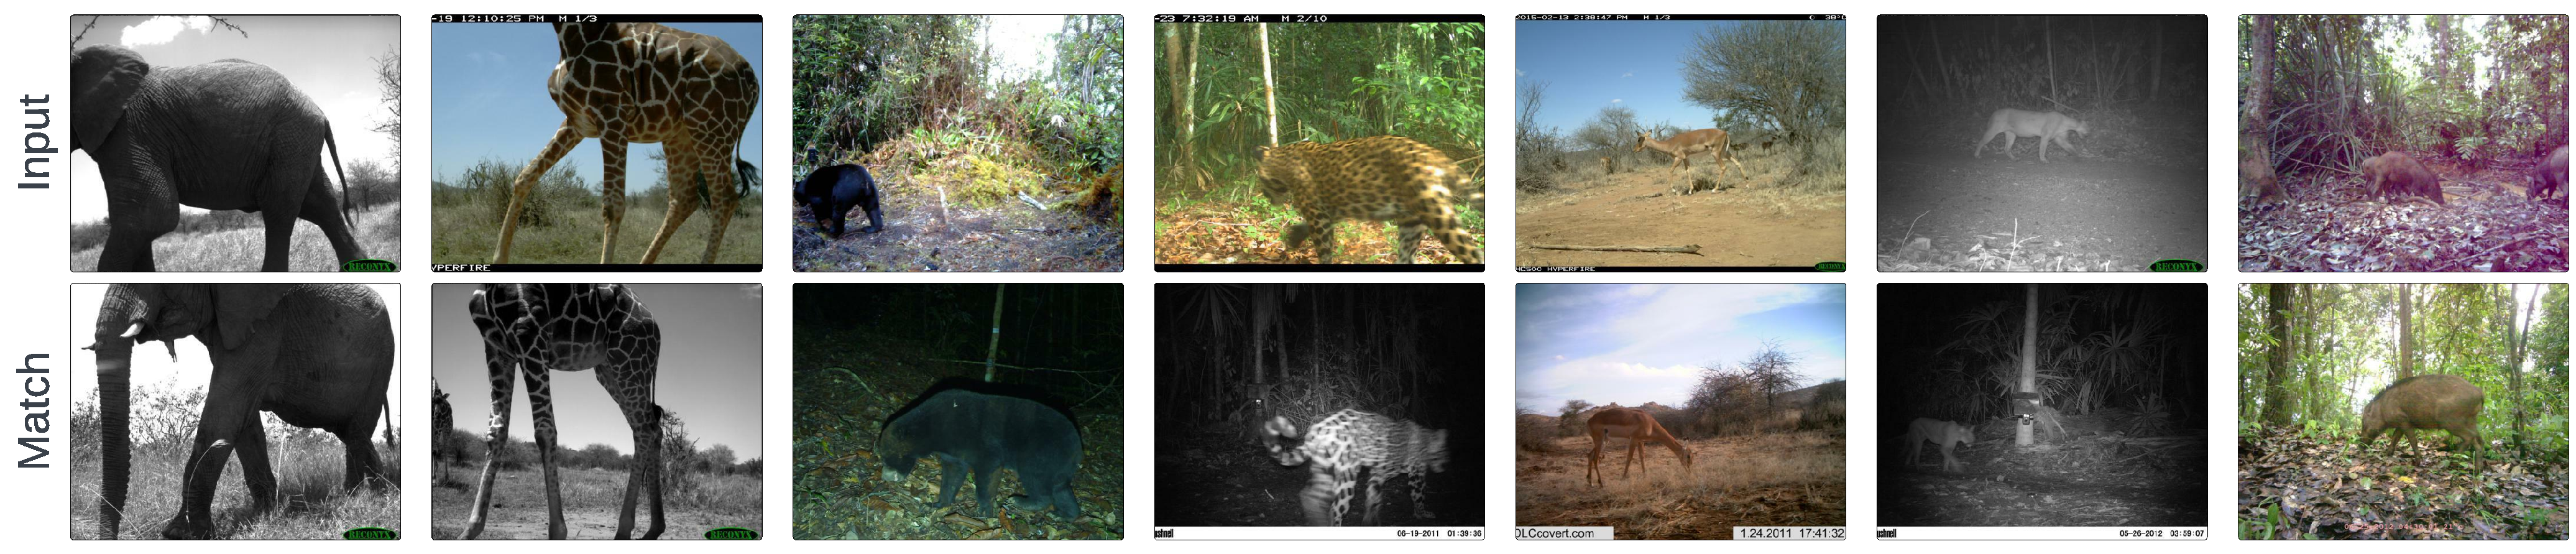
\includegraphics[width=1.\textwidth]{figures/matches_examples_2.pdf}
  \caption{
    %
    Examples of input (labelled) images and their 1-NN matched (unlabelled) images retrieved using
    \CNN{} on iWildCam dataset. 
    %
    Here, we match images from the labelled-train set to images from the unlabelled-extra set,
    taking advantage the fact that their domains are disjoint.
    %
  }
  \label{fig:matches_examples}
\end{figure}
